\documentclass{beamer}
\usepackage[utf8]{inputenc}
\usepackage[spanish]{babel}
\usepackage[T1]{fontenc}
\usepackage{amsmath,amssymb,amsfonts,amsthm}
\usepackage{graphicx}
\usepackage{tikz}

\usetheme{Madrid}
\usecolortheme{default}

\title[Temperatura de Curie]{Temperatura de Curie}
\subtitle{Una breve historia y aplicaciones físicas}
\author[Tu nombre]{Tu nombre}
\institute[Tu institución]{Tu institución}
\date{\today}

\begin{document}

\begin{frame}
    \titlepage
\end{frame}

\begin{frame}{Contexto histórico}
    \begin{itemize}
        \item La temperatura de Curie fue descubierta por Pierre Curie en 1895.
        \item Es la temperatura a la que un material ferromagnético pierde sus propiedades magnéticas.
        \item Pierre Curie descubrió este fenómeno mientras investigaba los cambios en la conductividad eléctrica de los materiales magnéticos a diferentes temperaturas.
        \item El descubrimiento de la temperatura de Curie fue fundamental en el desarrollo de la teoría del magnetismo y en la comprensión de las propiedades magnéticas de los materiales.
    \end{itemize}
\end{frame}

\begin{frame}{Definición matemática}
    \begin{equation*}
        \chi\left(T\right) = \frac{C}{T - \Theta_p}
    \end{equation*}
    \begin{itemize}
        \item $\chi(T)$: susceptibilidad magnética.
        \item $C$: constante de Curie.
        \item $\Theta_p$: temperatura de Curie.
        \item Esta ecuación describe cómo la susceptibilidad magnética de un material ferromagnético varía con la temperatura.
    \end{itemize}
\end{frame}

\begin{frame}{Aplicaciones físicas}
    \begin{itemize}
        \item La temperatura de Curie es importante en la fabricación de imanes.
        \item Permite determinar la temperatura máxima a la que un imán puede ser utilizado.
        \item También es relevante en la fabricación de dispositivos electrónicos, como los discos duros.
        \item La comprensión de la temperatura de Curie también ha llevado al desarrollo de nuevos materiales con propiedades magnéticas especiales.
    \end{itemize}
\end{frame}

\begin{frame}{Gráfica de la susceptibilidad magnética}
    \begin{figure}[h]
        \centering
        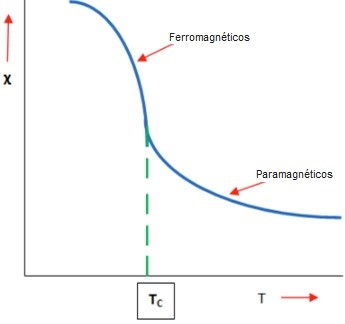
\includegraphics[width=0.6\textwidth]{curie-graph.jpg}
        \caption{Gráfica de la susceptibilidad magnética en función de la temperatura.}
        \label{fig:curie-graph}
    \end{figure}
\end{frame}

\begin{frame}{Contexto histórico}
    \begin{itemize}
        \item La temperatura de Curie fue descubierta por Pierre Curie en 1895.
        \item Junto a su esposa, Marie Curie, descubrieron el radio y recibieron el Premio Nobel de Física en 1903.
        \item Pierre Curie también hizo importantes contribuciones a la teoría de la magnetización, incluyendo la ley de Curie.
        \item La ley de Curie es una relación entre la temperatura y la susceptibilidad magnética de los materiales ferromagnéticos, y es un precursor de la temperatura de Curie.
    \end{itemize}
\end{frame}

\begin{frame}{Diferencia entre la ley de Curie y la ley de Curie-Weiss}
    \begin{itemize}
        \item La ley de Curie establece que la susceptibilidad magnética de los materiales ferromagnéticos es inversamente proporcional a la temperatura absoluta.
        \item La ley de Curie-Weiss es una extensión de la ley de Curie que tiene en cuenta la existencia de interacciones entre los momentos magnéticos en un material ferromagnético.
        \item La ley de Curie-Weiss establece que la susceptibilidad magnética es inversamente proporcional a la diferencia entre la temperatura absoluta y la llamada "temperatura de Curie-Weiss", que es una temperatura crítica que depende de las interacciones magnéticas del material.
        \item La ley de Curie-Weiss es una descripción más precisa del comportamiento de los materiales ferromagnéticos a temperaturas cercanas a la temperatura de Curie.
    \end{itemize}
\end{frame}

\begin{frame}{Diferencia entre la ley de Curie y la ley de Curie-Weiss}
    \begin{itemize}
        \item La ley de Curie describe la relación lineal entre la susceptibilidad magnética y la temperatura para materiales ferromagnéticos por debajo de la temperatura de Curie.
        \begin{equation*}
            \chi = \frac{C}{T - \theta}
        \end{equation*}
        \item La ley de Curie-Weiss describe la susceptibilidad magnética en función de la temperatura para materiales ferromagnéticos por encima de la temperatura de Curie. La ecuación se puede expresar como:
        \begin{equation*}
            \chi = \frac{C}{T - \theta} - \frac{C'}{T_C - T}
        \end{equation*}
        donde $T_C$ es la temperatura de Curie, $\theta$ es la temperatura de Weiss y $C$ y $C'$ son constantes.
    \end{itemize}
\end{frame}



\end{document}
